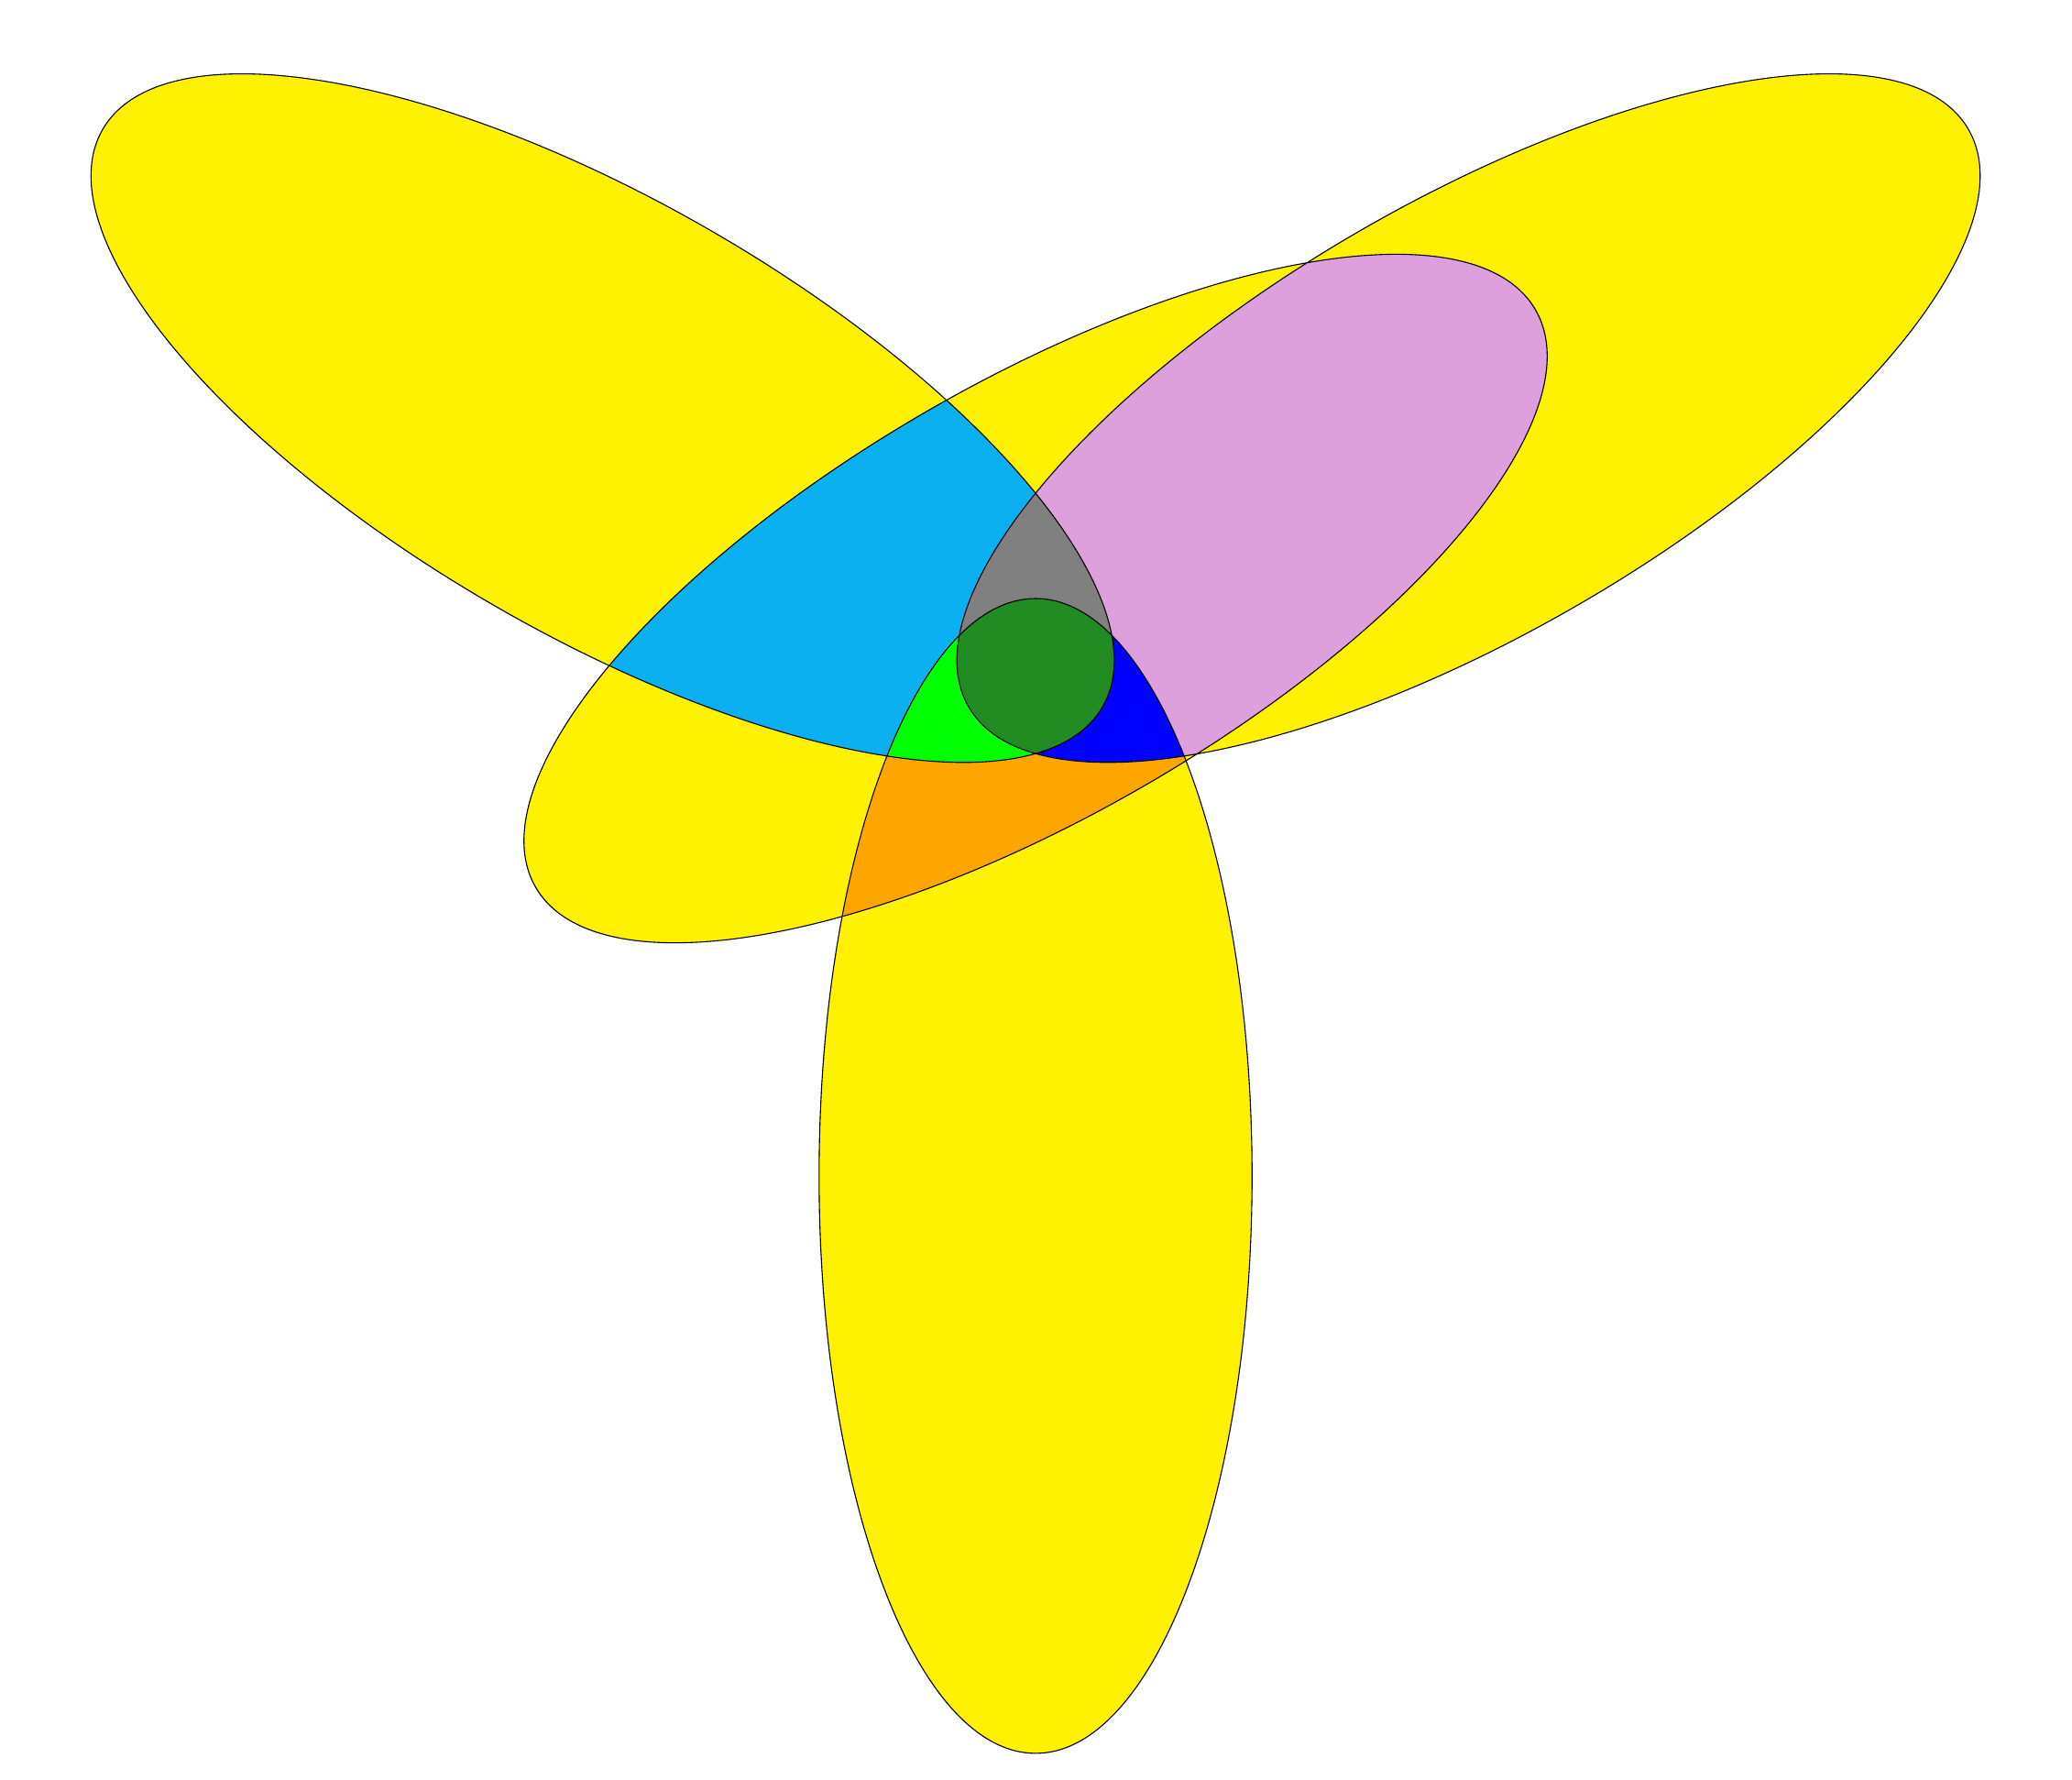
\begin{tikzpicture}
    \def\firstellipse{(-4,0) ellipse [x radius=8, y radius=3, rotate=150]}
    \def\secondellipse{(8,0) ellipse [x radius=8, y radius=3, rotate=30]}
    \def\thirdellipse{(2,-10.5) ellipse [x radius=8, y radius=3, rotate=90]}
    \def\fourthellipse{(2,-2.5) ellipse [x radius=8, y radius=3, rotate=210]}
    \def\boundingbox{(-12,-16) rectangle (16,3)}

    % fill ellipses
    \fill[yellow] \firstellipse \secondellipse \thirdellipse \fourthellipse;

    % fill intersections
    % intersection of second and third (2,3)
    \begin{scope}
        \clip \boundingbox \firstellipse;
        \clip \secondellipse;
        \fill[blue] \thirdellipse;
    \end{scope}
    % intersection of first and third (1,3)
    \begin{scope}
        \clip \boundingbox \secondellipse;
        \clip \firstellipse;
        \fill[green] \thirdellipse;
    \end{scope}
    % intersection of first and second (1,2)
    \begin{scope}
        \clip \boundingbox \thirdellipse;
        \clip \firstellipse;
        \fill[gray] \secondellipse;
    \end{scope}

    % (1,4)
    \begin{scope}
        \clip \boundingbox \thirdellipse;
        \clip \boundingbox \secondellipse;
        \clip \firstellipse;
        \fill[ProcessBlue] \fourthellipse;
    \end{scope}
    
    % (2,4)
    \begin{scope}
        \clip \boundingbox \firstellipse;
        \clip \boundingbox \thirdellipse;
        \clip \secondellipse;
        \fill[Plum] \fourthellipse;
    \end{scope}
    
    %(3,4)
    \begin{scope}
        \clip \boundingbox \firstellipse;
        \clip \boundingbox \secondellipse;
        \clip \thirdellipse;
        \fill[Orange] \fourthellipse;
    \end{scope}

    % intersection of first, second, third, and fourth
    \begin{scope}
        \clip \firstellipse;
        \clip \secondellipse;
        \clip \thirdellipse;
        \clip \fourthellipse;
        \fill[ForestGreen] \boundingbox;
    \end{scope}

    % outline of ellipses
    \draw \firstellipse \secondellipse \thirdellipse \fourthellipse;
\end{tikzpicture}